\subsection{Excercise UMEGeneralConcepts}
\label{sec:ume_general_concepts}
This task provides a general overview of the general concepts of the Unified Microservice Engineering (UME) approach.
The following sections will explain the general architectural style, the domain modeling process, and the modeling of the architecture.

\subsubsection*{Architectural Style}
The Unified Microservice Engineering approach aligns with the microservices architectural style.
This involves breaking down an application into smaller, independent services that can be developed, deployed, and scaled separately.
The services communicate with each other through APIs and are usually organized around business capabilities.
These services aim to enhance flexibility, scalability, and maintainability.

Predecessors of the microservices architectural style are the service-oriented architecture (SOA) and the distributed systems architectural style which will be further explained in the following.

\paragraph*{Service Oriented Architecture}
SOA shares some similarities with the microservices architectural style.
The focus is on organizing services around business capabilities and developing them independently.
This aims to achieve reusability and interoperability.

Yet, microservices tend to be generally smaller, more fine-grained, decoupled and are usually lightweight.

\paragraph*{Distributed Systems}
Distributed systems represent a collection of independent computers, appearing to the users of the system as a single coherent system.
These systems handle tasks across a network, each node having its local memory and set of responsibilities.

Microservices share a similar idea: Splitting an application into smaller, more independent services communicating with each other.
Each microservice manages its functionalities and data to provide the overall functionality of the application.

\subsubsection*{Domain Modelling}
Domain modeling is a UME approach that is part of the design phase.
Its goal is to create a domain model describing selected aspects of a domain.
However, the model should not separate the concept from the implementation.
It makes sure that the static and dynamic domain knowledge is used consistently by each feature.

The domain model is implemented in the domain logic layer of the layered architecture.
Therefore each domain microservice implements its domain model.

Therefore the domain logic layer is the part of the software architecture that is shaped the most by domain modeling.

\subsubsection*{Modelling of the Architecture}
To model the architecture of a microservice-based application, UME uses the Unified Modeling Language (UML).
To create the according diagrams, the UMLet tool \cite{UML-WEB} is used.

Two general views are distinguished: The Application Software View and the Application System View.
The application software view takes a logical approach and focuses on the software architecture.
It is represented by the Component Diagram.
The application system view takes a physical approach and focuses on the system architecture.
It is represented by the Deployment Diagram.

Both diagrams can be combined in the SystemPlusSoftware (SPS) Diagram.
It combines both the Component and the Deployment Diagram by putting the logical components into the physical nodes.

\subsection{Excercise APIStyles}
\label{sec:api_styles}
This task focuses on the different API styles used in the UME approach.
The following sections will explain ReST and gRPC and their properties, focusing on their usage, execution, similarities and differences.

\subsubsection*{ReST and gRPC}
\label{subsec:rest_and_grpc}
Two different API concepts are presented in this task: ReST and gRPC.

Representational State Transfer (ReST), is a popular architectural style for designing networked applications.
Five main properties are associated with ReST: Addressable resources, stateless communication, representation orientation, uniform and restricted interface, and format-driven state transfer.
It communicates using standard HTTP/HTTPS protocols, utilizing methods like \texttt{GET}, \texttt{POST}, \texttt{PUT}, and \texttt{DELETE}. 
Data interchange usually happens in JSON or XML format.
Due to the resource orientation, ReST is a good fit for CRUD operations.

gRPC Remote Procedure Call (gRPC), is an open-source framework developed by Google.
It is based on the idea of defining services and messages and specifying remotely callable methods.
gRPC uses data serialization with \texttt{protobuf}.
Communication happens via HTTP/2 since it offers streaming and multiplexing.
The data therefore is more lightweight and easier to store, however, it is less human-readable since it is binary.
Therefore, gRPC is a good fit for function-oriented microservice communication.

The main conceptual difference between REST and gRPC is their main focus and the way they implement their communication.
ReST is resource-oriented, focusing on the manipulation of resources, while gRPC is function-oriented.
REST is stateless using HTTP and JSON/XML, while gRPC uses HTTP/2 and \texttt{protobuf} for data serialization.
Therefore, one has to choose the API style that fits his requirements best.

\subsubsection*{ReST Properties}
ReST provides a concept of how microservices' APIs should be designed.
Its main properties are explained in the following.

To emphasize stateless communication, ReST requires the client to include all the information needed to process a request.
This simplifies sever design and allows for better stability.
Implementing a uniform restricted interface consistency in interactions is achieved.
This uniformity is enhanced by the use of URLs, HTTP methods, and representation orientation.
Lastly, ReST uses format-driven state transfer, meaning that the data is transferred in a specific format, usually JSON or XML.

\subsubsection*{gRPC Components}
% Name and describe the main components of the gRPC architecture.
gRPC is an open-source remote procedure call system, a competitive alternative to ReST.
As mentioned above, gRPC is based on the idea of defining services and specifying remotely callable methods.

\autoref{fig:grpc_main_components} from \cite{CM-T-DES} shows the main components that will be explained in the following.

\paragraph*{\texttt{.proto} File:}
The proto file defines the services, the messages, and the methods that can be called remotely.
Before calling a method, a stub needs to be generated.
This stub is generated from the \texttt{.proto} file and contains the method signatures.
The generation of the stub is done by the gRPC compiler.
This allows flexibility and independence of the used programming language.

\paragraph*{Client:}
The client is the caller of the remote methods.
It uses the stub to call the methods.
The communication between the client and the server uses \texttt{protobuf} messages via HTTP/2.
\texttt{protobuf} is Google's mechanism to serialize data, making data more lightweight and easier to store, persist and transfer.
More on this topic can be found in the official documentation: \url{https://protobuf.dev/overview/}.

\paragraph*{Server:}
The server is the receiver of the remote method calls.
It holds the functions defined as services in the \texttt{.proto} file.
After receiving a call, the server executes the method and returns the result to the client, again via HTTP/2.

\begin{figure}
    \centering
    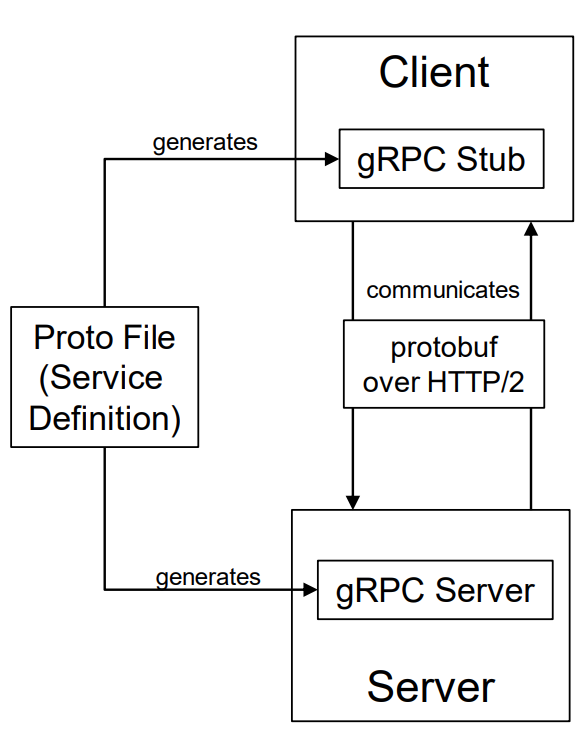
\includegraphics[width=0.4\textwidth]{figures/microservices/microservices_grpcMainComponents.png}
    \caption{Main Components of the gRPC Architecture}
    \label{fig:grpc_main_components}
\end{figure}

\subsubsection*{Use of ReST and gRPC in UME}
% Which API style is appropriate for which type of microservice in the UME approach?
Each API style applies to different use cases and microservice types.
Taking a look at a standard DDD-based layered architecture, splitting the logic layer into application and domain logic, different API styles can be used for each logic layer.
Two microservice types, namely domain microservices (DM) and application microservices (DM), are distinguished in the UME approach.
Usually, gRPC is suitable for application microservices, while ReST is suitable for domain microservices.

\subsection{Excercise ArchitectureCarRentalAppV1.0}
\label{sec:architecture_car_rental_app_v1_0}
\subsubsection*{Documentation Repository}
The documentation repository can be found at \url{https://gitlab.kit.edu/kit/cm/teaching/carrentalapp/0.doccarrentalappv1}.
It is called \texttt{0.DocCarRentalAppV1} and contains the documentation of the Car Rental App V1.0.
It comprises three directories and a \texttt{README.md} file.
The structure is shown in \autoref{fig:doc_repo_car_rental_app_v1}.
The folders are structured as follows:

\paragraph*{Figures:}
This folder contains all the figures representing the component-, architecture-, systemPlusSoftware -, and deployment diagrams.
It contains the first and second versions of each diagram respectively.
The figures are stored as \texttt{.png} files.
These files are then used in the documentation.
\paragraph*{Pages:}
This folder contains all the pages of the documentation.
They are kept in separate markdown files for better readability and maintainability.
Most of them also are structured into first and second versions respectively.
The readme file in the root folder links to the pages stored in this folder if there is a reference.
\paragraph*{Umlet:}
This folder contains the UMLet files of the diagrams.
These files are stored as \texttt{.uxf} files and can therefore be edited using the UMLet tool.
The figures folder holds the exported images of the diagrams from this folder.
It also holds a \texttt{.gitkeep} file to keep the folder in the repository even if it is empty.

\begin{figure}
    \centering
    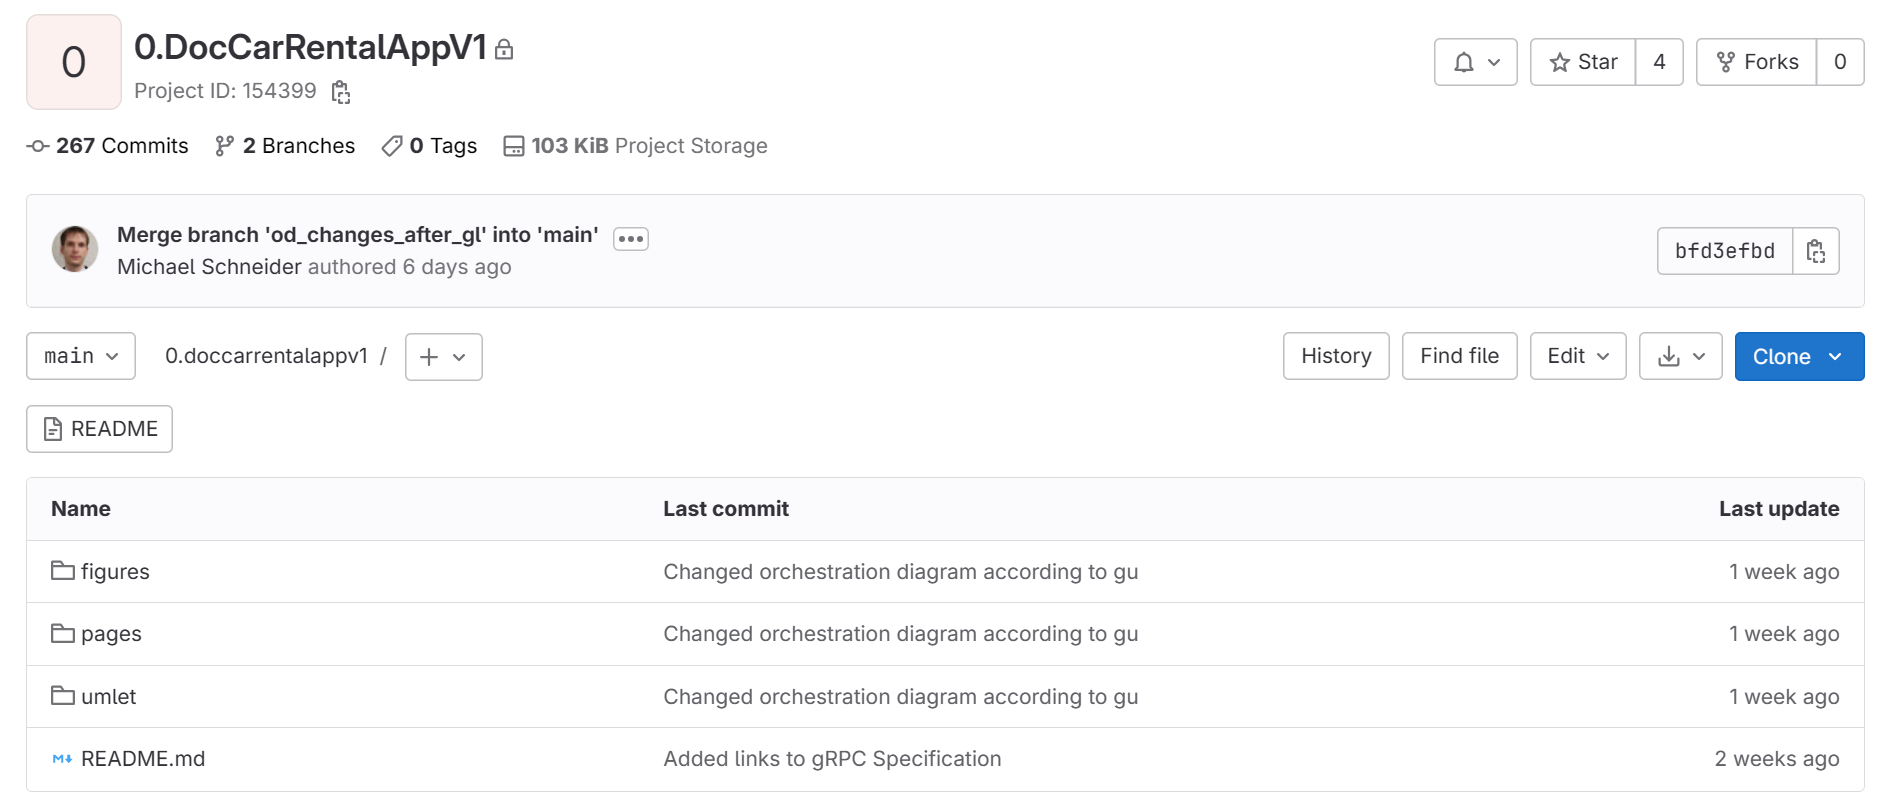
\includegraphics[width=\textwidth]{figures/microservices/introduction/ms_intro_docRepo.png}
    \caption{Documentation Repository of the Car Rental App V1.0}
    \label{fig:doc_repo_car_rental_app_v1}
\end{figure}

\subsubsection*{Type of Architecture and Diagram}
As mentioned above, the diagrams can be found exported as images in the figures folder and as UMLet files in the UMLet folder.
Therefore the architecture diagram can be found in \texttt{0.doccarrentalappv1/figures/ad\_dm-car\_v1.0.png} and \hfill \linebreak \texttt{0.doccarrentalappv1/umlet/cd\_car\_rental\_app\_v1.0.uxf} respectively.
It is a component diagram, showing the components representing the different layers of the architecture and their dependencies.
They can be separated into the presentation layer (UI), the application logic layer (application microservice), the domain logic layer (domain microservice), and the infrastructure layer (databases).

\subsubsection*{Extension of the Architecture}
\texttt{CarRentalAppV1.0}'s deployment diagram is shown in \autoref{fig:system_plus_software_car_rental_app_v1}.
Each component is deployed as a separate and independent microservice.
The deployment is defined by a dedicated Docker file.
These files specify dependencies and the overall environment for each component.
Therefore, each component can be containerized and deployed seamlessly within the same Kubernetes cluster.
Each cluster can be hosted on any chosen cloud provider.
This gives a certain flexibility in terms of deployment options.

\begin{figure}
    \centering
    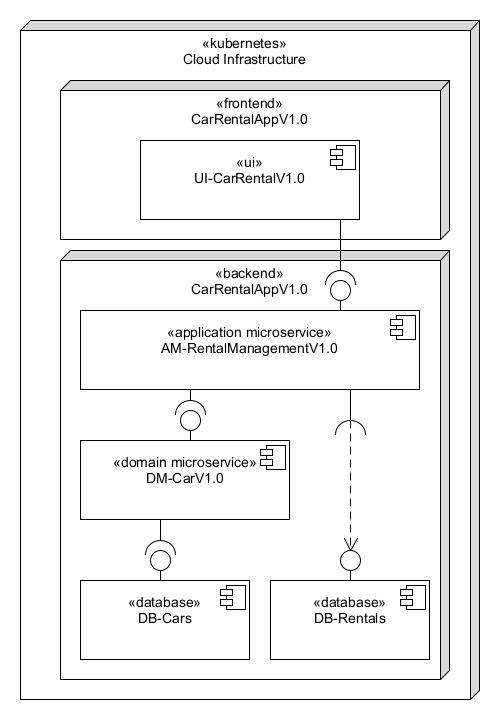
\includegraphics[width=0.5\textwidth]{figures/microservices/introduction/ms_dmCar_SPScarRental.png}
    \caption{SystemPlusSoftware Diagram of the Car Rental App V1.0}
    \label{fig:system_plus_software_car_rental_app_v1}
\end{figure}
